%\begin{itemize}
%	\item definition of the dialect construction
%	\item hiding operation, free pseudo-trace
%\end{itemize}


The first step of the construction is, starting with a SMC, to equip morphisms with a notion of
\emph{state} or \emph{private space}. As the name suggests, when composing two such morphisms
the private parts will avoid each other and not interact. The basic idea here is that any interface
in the private space is unerstood as \emph{virtually} traced and subjected to the trace equations.
We detail and formalize this in the following definition.

\begin{definition}[state pseudo-category]
	Let $\catf C$ be a symmetric monoidal category. Define $\state C$ the \emph{state 
	pseudo\footnotemark-category}
	over $\catf C$ as:
	\begin{itemize}
		\item The objects of $\state C$ are those of $\catf C$.
		\item A morphism from $A$ to $B$ in $\state C$ is a pair $(f,U)$,
		where $U$ is an object of $\catf C$ and $\morph f{A\monp U}{B\monp U}$ is a morphism of 
		$\catf C$.
		\item The identity on $A$ is defined as the pair $(\Id_A, \unitobj)$.
		\item Composition of morphisms $\morph{(f,U)}{A}{B}$ and $\morph{(g,V)}{B}{C}$ is defined by
		$$(f,U)\sq(g,V)=\big(\:
		( f\monp V)\sq(B\monp \symm UV)\sq(g\monp U)\sq(C\monp\symm VU)
		\:,\,U\monp V\,\big)$$
		\FIGURE{composition}
	\end{itemize}
\end{definition}
\footnotetext{Composition does not necessarily satisfy associativity yet.}

Unless $\catf C$ is strict, $\state C$ will not be a proper category in general: if we have objects
such that $U\monp (V\monp W)\neq (U\monp V)\monp W$ then morphisms
$(f,U) \sq \big((g,V) \sq (h,W)\big)$ and $\big((f,U) \sq (g,V)\big) \sq (h,W)$ cannot be equal.
However, everything becomes  perfectly fine if we look at state-equiped morphisms 
\emph{up to sliding isomorphisms}, one of the trace equations. This leads to the definition of the
\emph{dialect category}, the name dialect paying tribute to a similarly named construction introduced
by J.-Y. Girard in his work on geometry of interaction~\cite{girard95}.

\begin{definition}[dialect category]
	The \emph{dialect category} $\dial C$ over $\catf C$ is defined by quotienting morphisms of
	$\state C$ by the following equivalence relation, which we call \emph{sliding equivalence}:
		$$\big(\,f\sq(B\monp\phi)\,,\,U\,\big)\eq \big(\,(B\monp\phi)\sq f\,,\,V\,\big) \text{ \ for any 
		$\catf C\!$-isomorphism\footnotemark $\morph\phi VU$ and 
		$\morph f{A\monp U}{B\monp V}$}
		$$
		\FIGURE{sliding in state category}
		\footnotetext{One could choose to allow sliding of \emph{any} morphisms here.
		But in the presence of yanking one can recover the full case where $\phi$ is any
		morphism from the isomorphism case~\cite{jsv96}. Moreover sliding only isomorphisms is 
		enough to make $\dial C$ a category and isomorphisms are more convenient to manipulate.
		}
\end{definition}

Once this definition is set up, it is an easy exercise to check that the composition operation
becomes associative in $\dial C$ and that the $(\Id_A, \unitobj)$ are neutral.

\begin{proposition}
	After quotienting, $\dial C$ is indeed a category.
\end{proposition}

\begin{proposition}
	There is a functorial embedding $\embd C$ of $\catf C$ into $\dial C$ defined as the identity on
	objects and $\embd C (f)=(f\monp \Id_{\unitobj}, \unitobj)$ on morphisms.
\end{proposition}

\begin{proof}
	The fact that $\embd C(f\sq g)=\embd C(f) \sq \embd C(g)$ follows readily from the structure
	equations involving $\unitobj$. Then, if $\embd C(f) \eq \embd C(g)$, this means that there
	exist $\morph{f'}{A\monp \unitobj}{B\monp \unitobj}$, 
	$\morph{g'}{A\monp \unitobj}{B\monp \unitobj}$ and an isomorphism $\morph\phi\unitobj\unitobj$
	such that $f\monp\Id_\unitobj=f'\sq (\Id_B\monp\phi)$ and 
	$g\monp\Id_\unitobj=(\Id_A\monp\phi)\sq g'$. General properties of morphisms from $\unitobj$ to
	$\unitobj$ in monoidal categories imply that, for instance, $(\Id_A\monp\phi)\sq g'=g'\sq (\Id_B\monp\phi)$,
	so that $f'=g'$ and eventually $f=g$.
\end{proof}

Moreover the monoidal structure of $\catf C$ can be lifted to $\dial C$.

\begin{proposition}[monoidal structure]
	We can define the following monoidal structure on $\dial C$:
	\begin{itemize}
		\item The unit object $\unitobj$ is the one from $\catf C$.
		\item The bifunctor $\monp$ is defined the same way on objects and as follows on morphisms:
		$$(f,U)\monp(g,V)=(A\monp \symm CU\monp V)\sq(f\monp g)\sq(B\monp \symm UD\monp V)
		$$
		(with $\morph f{A\monp V}{B\monp V}$ and $\morph g{C\monp V}{D\monp V}$)
		\item All the structure isomorphisms are obtained \via the embedding $\embd C$, \eg the
		symmetries are defined as $(\symm AB, \unitobj)$.
	\end{itemize}
\end{proposition}

\begin{proof}
	We first have to make sure that the new $\monp$ is well-defined, \ie that it is compatible with
	$\eq$, explicitely: whenever $(f,U)\eq(g,V)$ then for any $(h,W)$ we have 
	$\big((h,W)\monp(f,U)\big)\eq\big((h,W)\monp(g,V)\big)$ and 
	$\big((f,U)\monp(h,W)\big)\eq\big((g,V)\monp(h,W)\big)$ which follows immediately after carefully
	unfolding the definitions.

	Because we defined the structure isomorphisms using a functorial embedding, all the needed
	structure equations carry over to $\dial C$. The only thing remaining to check is whether
	the families of structure isomorphisms thus defined are still natural.
	Let us look at the case of symmetries to see what type of computation we are dealing with. The
	other cases are similar.
	
	\FIGURE{graphical computation}
\end{proof}

Now that we have this general context to work in, we can already remark something interesting:
if we have a morphism $\morph{(f,V)}{A\monp U}{B\monp U}$ in $\dial C$ (that is, a morphism
$\morph f {A\monp U\monp V}{A\monp U\monp V}$ in $\catf C$) there is a natural operation that can be
performed which resembles taking a trace, at least at the level of interfaces: one can push $U$
to the private part of $f$, making it a morphism from $A$ to $B$ in $\dial C$.

\begin{definition}[Hiding]
	Given a morphism $\morph{(f,V)}{A\monp U}{B\monp U}$ of $\dial C$, define 
	$$\hide U[f,V]=(f,U\monp V)$$
	We call this operation \emph{hiding $U$}.
\end{definition}

This operation not only shares the action on interfaces of a trace, it also has most of the required
properties of traces. Most notably since we defined $\dial C$ \via making sliding equations into equalities,
it satisfies sliding. Even more than that, the pseudo-trace structure obtained is the free one.

\begin{theorem}[free pseudo trace]
	The hiding operation $\hide{}[\cdot]$ defines a pseudo-trace (\ie a trace minus yanking)
	in $\dial C$.
	Moreover, $\dial C$ satisfies the following universal property: for any pseudo-traced
	category $\catf D$ and monoidal functor $\morph F{\catf C}{\catf D}$ we have that $F$
	factors uniquely as 
	\begin{center}
	$\funcf F=\funcf G\circ \embd C$ \qquad\qquad
	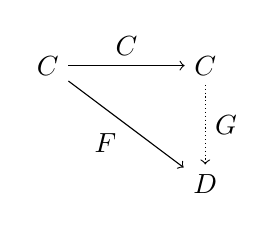
\begin{tikzpicture}[baseline=-5ex]
		\node (c) at (0,0) {$\catf C$};
		\node (tc) at (2,0) {$\dial C$};
		\node (d) at (2,-1.5) {$\catf D$};
		\draw[->] (c) to node [above] {$\embd C$} (tc);
		\draw[->] (c) to node [below left] {$\funcf F$} (d);
		\draw[->,densely dotted] (tc) to node [right] {$\funcf G$} (d);
	\end{tikzpicture}
\end{center}
	with $G$ a pseudo-traced functor.
\end{theorem}

\begin{proof}
\TODO{More detailed proof than in my short note.}
%	Set $G(f,U)=\Tr{\funcf FU}[\funcf F f]$ (this is well defined because $\Tr{}$ satisfies sliding)
%	with structure maps being those of $F$.
%	It factors $F$ because of vanishing and $\funcf F\unitobj\simeq\unitobj$, and is indeed a
%	pseudo-traced functor because we defined it using $\Tr{}$.
%	
%	An easy computation gives the unicity property.
\end{proof}

%\begin{remark}
%	This universal property implies that $\dial \cdot$ is a functor.
%\end{remark}



